\documentclass[12pt, a4paper]{report}
\setcounter{secnumdepth}{0}
\usepackage{graphicx}
\usepackage{titlesec}
\usepackage{pdfpages}
\usepackage{wrapfig}
\usepackage[T1]{fontenc}
\usepackage[utf8]{inputenc}
\graphicspath{ {./images/} }

\title{
  \begin{huge}
    \textbf{
      {Computer Science Project 2020-'21}\\
      {Sudoku Web App}
    }\\
  \end{huge}
  \begin{figure}
      \centering
      {
\includegraphics[scale=2]{iss}}
  \end{figure}
}
\author{
x % add only one name here
}

\date{\vspace{-5ex}}

\begin{document}

  \begin{titlepage}
  \maketitle
  \end{titlepage}

  \newpage
  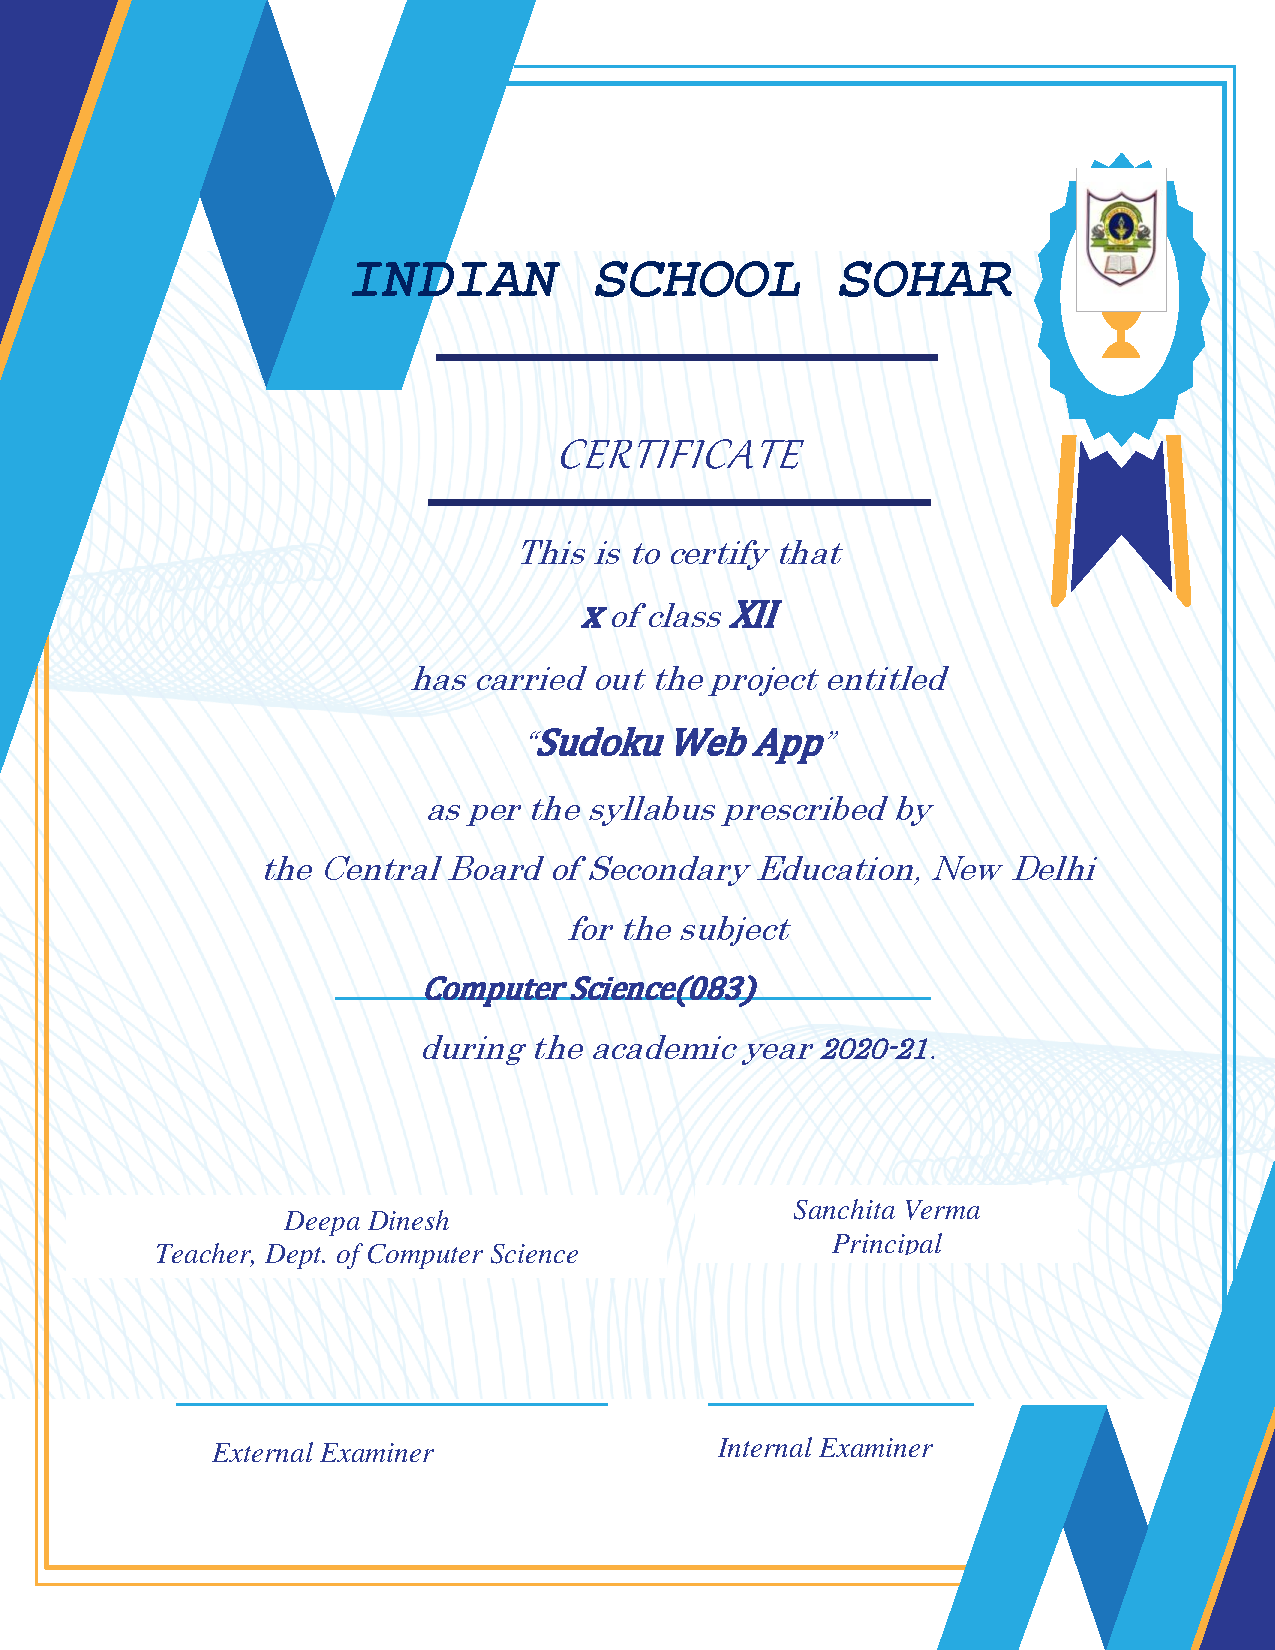
\includepdf{cert}
  
  \newpage
  \maketitle
  \begin{large}
  \section*{Acknowledgements}
  I have taken efforts in this project. However, it would not have been possible without the kind support and help of many individuals and organizations. I would like to extend my sincere thanks to all of them. \newline
  \newline
  I am greatly indebted to the teacher-in-charge, Ms.~Deepa Dinesh for her guidance and constant supervision as well as for providing necessary information 
  regarding the project and also for her support in completing the project. \newline
  \newline
  I would like to express my gratitude towards my parents for their kind cooperation and encouragement which helped me in the completion of this project. \newline
  \newline
  I would also like to express my special gratitude and thanks to my classmates in developing the project and to the people who have willingly 
  helped me out with their abilities.
  \end{large}
 
  \maketitle
  \begin{large}
  \newpage
  \tableofcontents
  \end{large}
  
  \newpage
  \section{Introduction}
  Python was created in the late 1980s, and first released in 1991, by Guido van Rossum as a successor to the ABC programming language.
  \begin{wrapfigure}{r}{0.25\textwidth}
    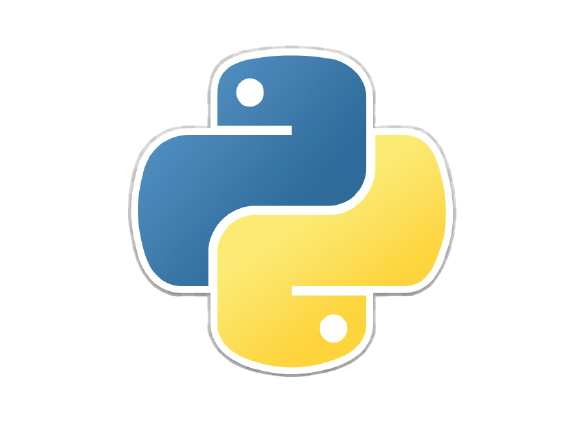
\includegraphics[width=0.25\textwidth]{introduction}
  \end{wrapfigure}
  Python is an interpreted, object-oriented, high-level programming language with dynamic semantics. Its high-level built in data structures, combined with dynamic typing and dynamic binding, make it very attractive for Rapid Application Development, as well as for use as a scripting or glue language to connect existing components together.

  Python's simple, easy to learn syntax emphasizes readability and therefore reduces the cost of program maintenance. Python supports modules and packages, which encourages program modularity and code reuse. The Python interpreter and the extensive standard library are available in source or binary form without charge for all major platforms, and can be freely distributed.
  
  \subsection{Features in Python:}
    \subsubsection{Easy to code:}
    Python is a high-level programming language. Python is very easy to learn as compared to other languages like C, C#, JavaScript, Java, etc. It is very easy to code in python language and anybody can learn python basics in a few hours or days. It is also a developer-friendly language.
    
    \subsubsection{Free and Open Source:}
    Since it is open-source, this means that source code is also available to the public. So you can download it as, use it as well as share it.
    
    \subsubsection{Object-Oriented Language:}
    One of the key features of Python is Object-Oriented Programming. Python supports object-oriented language and concepts of classes, objects, encapsulation, etc.
    
    \subsubsection{High-Level Language:}
    Python is a high-level language. When we write programs in Python, we do not need to remember the system architecture or manage memory.
    
  \newpage
  \section{Feasibility Study}
   yes
  
  \newpage
  \section{Hardware and Software}
   Add stuff here
  
  \newpage
  \section{About the Project}
  About the project
  
  \newpage
  \section{Source Code}
  Add a code overview here.
  
  \newpage
  \section{Bibliography}
  Add final output result here.
  
\end{document}
